\chapter{Résultats}

\section{Introduction}
Afin d’avoir un jeu de données assez riche, varié et aussi complet que possible et surtout réaliste, j’ai dû passer par plusieurs entreprises, essuyer plusieurs refus en raison de la confidentialité et de la protection des informations des salariés, pour parvenir à me procurer une liste anonyme d’une dizaine de salariés qui me servira de base de travail.

\section{Le jeu de données pour le test :}
Ce sont les résultats des salariés de l’entreprise du semestre passé qui m'ont permis d'élaborer la matrice de décision sous forme du « tableau des performances » ci-dessous : 

\begin{figure}[!h]
\begin{center}
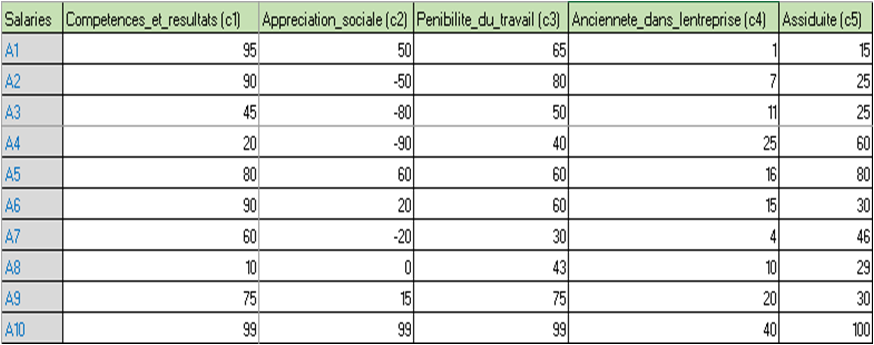
\includegraphics{Tests_resultats/performances_salaries.png}
\end{center}
\caption{tableau des performances des salariés}
\end{figure}

\section{Les résultats :}
Pour vérifier les résultats de mon programme sur cette matrice, j’ai comparé mes résultats obtenus avec l’application des deux méthodes «la méthode de la somme pondérée et la méthode ELECTRE III » avec le cas réel, c’est-à-dire les salariés qui ont réellement reçu une promotion à la fin du semestre dernier au sein de l’entreprise.
\newpage

\begin{itemize}
\item Le classement des salariés d’après l’entreprise :
\begin{figure}[!h]
\begin{center}
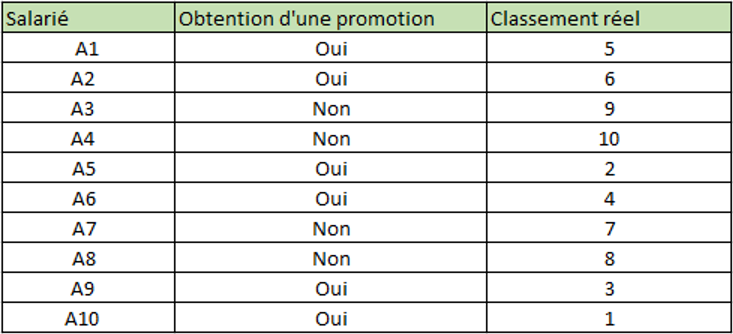
\includegraphics{Tests_resultats/classement_salarie.png}
\end{center}
\caption{classement des salariés d’après l’entreprise}
\end{figure}

\item Le classement des salariés avec la méthode de la somme pondérée
\begin{figure}[!h]
\begin{center}
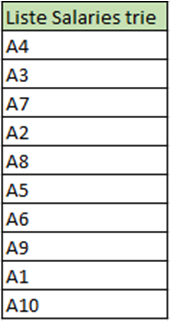
\includegraphics{Tests_resultats/classement_somme_pondere.png}
\end{center}
\caption{résultat du classement des salariés avec la méthode de la somme pondérée}
\end{figure}

\item Le classement des salariés avec la méthode ELECTRE III
\begin{figure}[!h]
\begin{center}
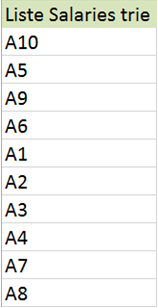
\includegraphics{Tests_resultats/classement_electre.png}
\end{center}
\caption{résultat du classement des salariés avec la méthode ELECTRE III}
\end{figure}

\section{Explication des résultats :}
D’après les résultats obtenus, on remarque clairement que le résultat affiché avec la méthode ELECTRE se rapproche de manière considérable du classement réel des salariés de l’entreprise, contrairement au résultat obtenu avec la méthode de la somme pondérée qui, elle, affiche un résultat diffèrent.\\
Ces résultats s’expliquent du fait que la méthode ELECTRE est plus adaptée pour les analyses d’aide à la décision multicritère où on a de nombreux critères qui entrent en jeu. Quant à la méthode de la somme pondérée ses résultats sont plus efficaces quand on considère un seul critère par exemple « si le salarié a atteint ou pas son objectif » ce qui est fait dans la méthode MBO. 


\section{Conclusion :}
Dans ce chapitre on a présenté tout d’abord, les tests effectués ainsi que les résultats obtenus suite à l’application des deux méthodes d’analyses multicritères « la Somme pondérée et ELECTRE III » sur les données de performances des salariés. Puis, on a effectué une comparaison des résultats obtenus. Dans le chapitre suivant seront développées les perspectives ainsi que la conclusion.
\end{itemize}
